\documentclass[a4paper,10pt,titlepage]{article}

\usepackage{geometry}
\usepackage{amsmath}
\usepackage{amssymb}
\usepackage{txfonts}
\usepackage{microtype}
\usepackage{epsfig}
\usepackage{graphicx}
\usepackage{moreverb}
\usepackage{hyperref}
\usepackage{listings}
\usepackage{xcolor}
\usepackage{textcomp}
\definecolor{listinggray}{gray}{0.98}
\definecolor{lbcolor}{rgb}{0.98,0.98,0.98}
\lstset{
	backgroundcolor=\color{lbcolor},
	tabsize=4,
	rulecolor=,
	language=matlab,
    basicstyle=\scriptsize\ttfamily,
    upquote=true,
    aboveskip={1.5\baselineskip},
    columns=fixed,
    showstringspaces=false,
    extendedchars=true,
    breaklines=true,
    prebreak = \raisebox{0ex}[0ex][0ex]{\ensuremath{\hookleftarrow}},
    frame=single,
    showtabs=false,
    showspaces=false,
    showstringspaces=false,
    identifierstyle=\ttfamily,
    keywordstyle=\color[rgb]{0,0,1},
    commentstyle=\color[rgb]{0.133,0.545,0.133},
    stringstyle=\color[rgb]{0.627,0.126,0.941},
}
\usepackage{eso-pic}
\usepackage{ifthen}

\AddToShipoutPictureBG{\ifthenelse{\equal{\value{page}}{0}}{}{
\includegraphics{template_files/backgroundlines}}}

\usepackage{units}
%\usepackage[T1]{fontenc}
%\usepackage[utf8]{inputenc}
\usepackage{physics}

\newcommand{\ee}{\mathrm{e}}
\newcommand{\ii}{\mathrm{i}}

\title{H2a: Binary Alloy}
\author{Andr\'eas Sundstr\"om and Linnea Hesslow}
\date{\today}

\begin{document}

\newgeometry{top=2cm,bottom=2cm,left=2cm,right=2cm}

\begin{titlepage}

\setcounter{page}{0}

\begin{center}
{\huge \bf \color{red} NB: The graded, first version of the report must be
                           returned if you hand in a second time! } \\
\vspace{3cm}
\makeatletter
{ \huge \@title } \\
\vspace{1cm}
{ \Large \@author }\\
\vspace{1cm}
{ \Large \@date }\\
\makeatother
\end{center}

\vfill

\begin{flushright}
{\Large
\begin{tabular}{|c|c|c|}
\hline
Task N\textsuperscript{\underline{o}} & Points & Avail.\ points \\ \hline
\hspace{3cm} & \hspace{3cm} & \hspace{3cm} \\ \hline
~ & ~ & ~ \\ \hline
~ & ~ & ~ \\ \hline
~ & ~ & ~ \\ \hline
~ & ~ & ~ \\ \hline
~ & ~ & ~ \\ \hline
~ & ~ & ~ \\ \hline
~ & ~ & ~ \\ \hline
$\sum$ & ~ & ~ \\
\hline
\end{tabular}}
\end{flushright}

\end{titlepage}

\newgeometry{top=2cm,bottom=2cm,left=1.5cm,right=7.4cm}


\section*{Introduction}
We study a simple model of a binary alloy of copper and zink, commonly known as brass. Some properties of the system can be determined analytically in the mean field theory, but a numerical simulation of the Ising model gives more accurate results at low dimensionality. Both the mean field theory and the Ising model play an important role in statistical mechanics. We use these two models to compute various statistical properties and compare the results. 

\section*{Task 1: mean field theory}
Fits: we obtained $\alpha \approx 0.494$

\begin{figure}[!ht]
\begin{center}
  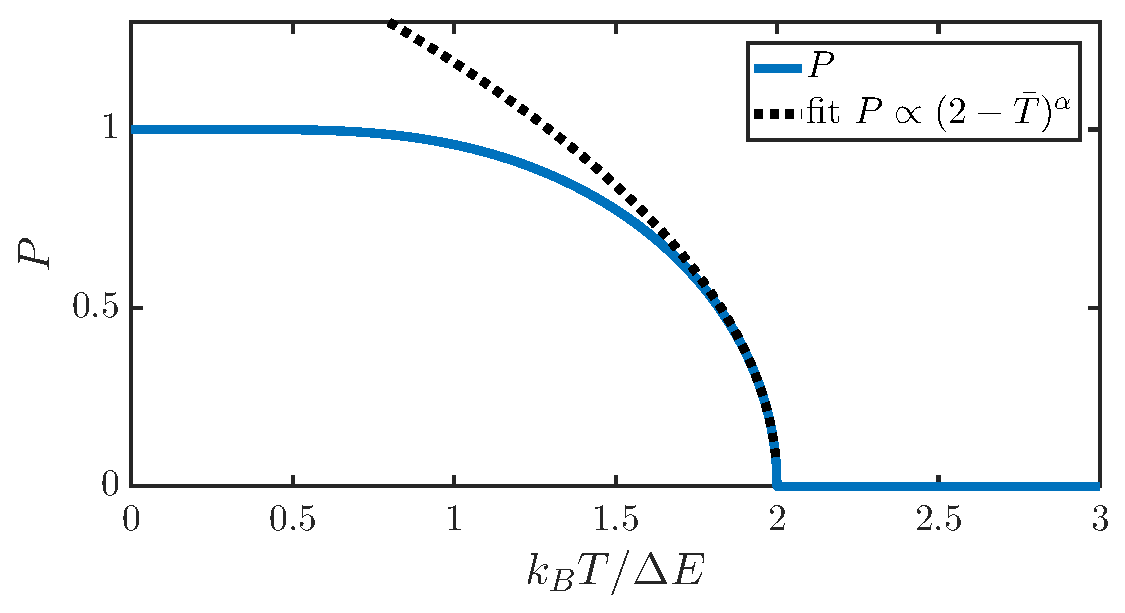
\includegraphics[width=0.7\textwidth]{../figures/P_MFT} 
  \caption{.....}
  \label{fig:T1:P}
\end{center}
\end{figure}

\begin{figure}[!ht]
\begin{center}
  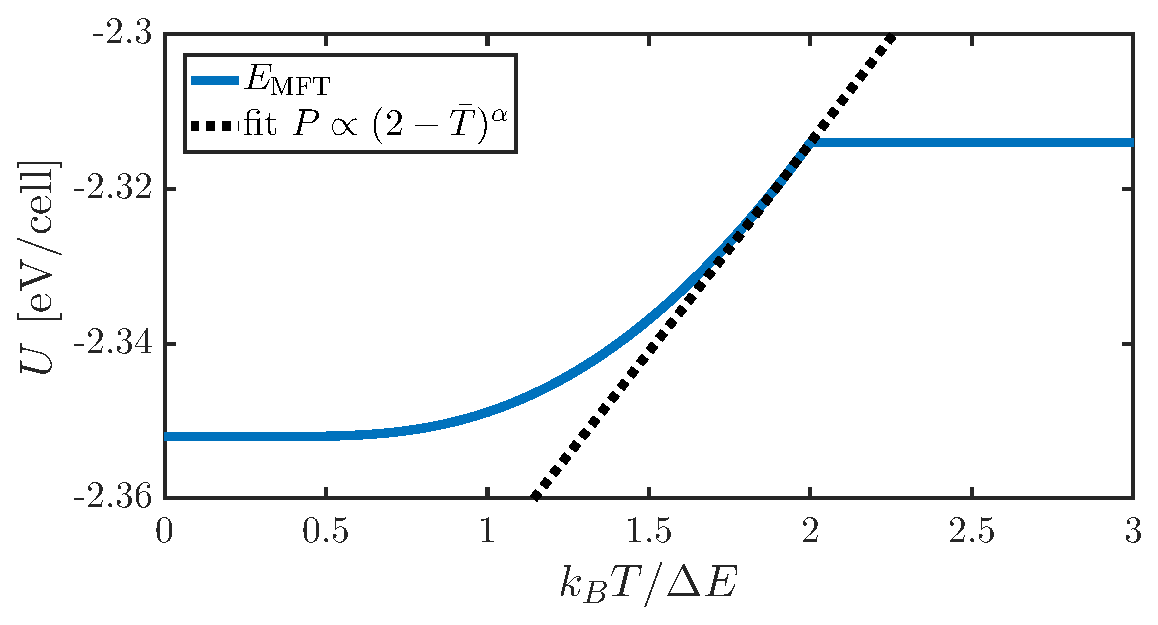
\includegraphics[width=0.7\textwidth]{../figures/E_MFT} 
  \caption{......}
  \label{fig:T1:E}
\end{center}
\end{figure}

\begin{figure}[!ht]
\begin{center}
  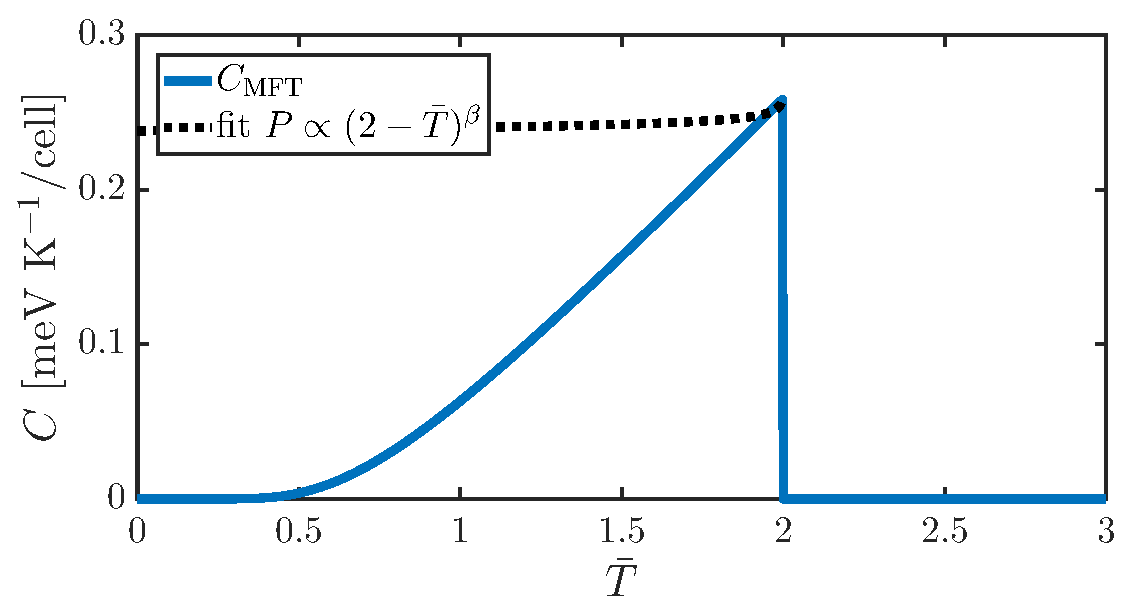
\includegraphics[width=0.7\textwidth]{../figures/C_MFT} 
  \caption{......}
  \label{fig:T1:C}
\end{center}
\end{figure}

%%%%%%%%%%%%%%%%%%%%%%%%%%%%%%%%%%%%%%%%%%%%%%%%%%%%%%%
\section*{Task 2: Ising model}

We model the binary alloy with a static bcc lattice consisting of Cu and Zn atoms. The system size was $10 \times 10 \times 10$ cells and had periodic boundary conditions. Each atoms has eight bonds to each nearest neighbors, with energies
\begin{equation}
\begin{aligned}
E_{\rm CuZn} &= \unit[-294]{meV} \\
E_{\rm CuCu} &= \unit[-436]{meV} \\
E_{\rm ZnZn} &= \unit[-133]{meV}
\end{aligned}
\label{eq:energies}
\end{equation}
We use the Metropolis algorithm to estimate statistical properties of the system. In each simulation step, we swap two randomly selected atoms in the lattice, and determine the energy change $\Delta E$. If $\Delta E \leq 0$, or if $(\exp[-\Delta E/(k_{\rm B} T)] > \xi$, where $\xi$ is a random number between $0$ and $1$, the change is accepted; otherwise the lattice remains in the previous state for another timestep. In this way, the Metropolis algorithm allows us to sample the state space according to the probability function $p \propto \exp[- E/(k_{\rm B} T)]$, and thus favor the most probable configurations. 

\subsection*{Equilibration}
To equilibrate the system, we started with an ordered system and performed $N_{\rm eq, long} = 10^6$ Monte Carlo steps to equilibrate the system at $T = \unit[-200]{^\circ C}$. At higher temperatures, we started with the final lattice state of the previous temperature, and therefore the number of equilibration steps was reduced to $N_{\rm eq, short} = 5 \cdot 10^5$. For all temperatures, we used $10^7$ Monte Carlo steps in the production run. 

Figure~\ref{fig:T2:equil} shows the equilibration of the energy at three different temperatures: significantly below, close to and significantly above the critical temperature $T = \unit[440]{^\circ C}$. By plotting the energy per bond, i.e.\  $E/(8 N_{\rm Cu})$, we can compare the energies to the binding energies in equation~\eqref{eq:energies}. 
We note that the energy per bond is in the range $E_{\rm CuZn} \leq E \leq E_{\rm max}$, where
\begin{equation}
 E_{\rm max} \equiv \frac{1}{2}(E_{\rm CuCu} + E_{\rm ZnZn}) = \unit[-284.5]{meV}.
 \label{eq:Emax}
\end{equation}

\begin{figure}[!ht]
\begin{center}
  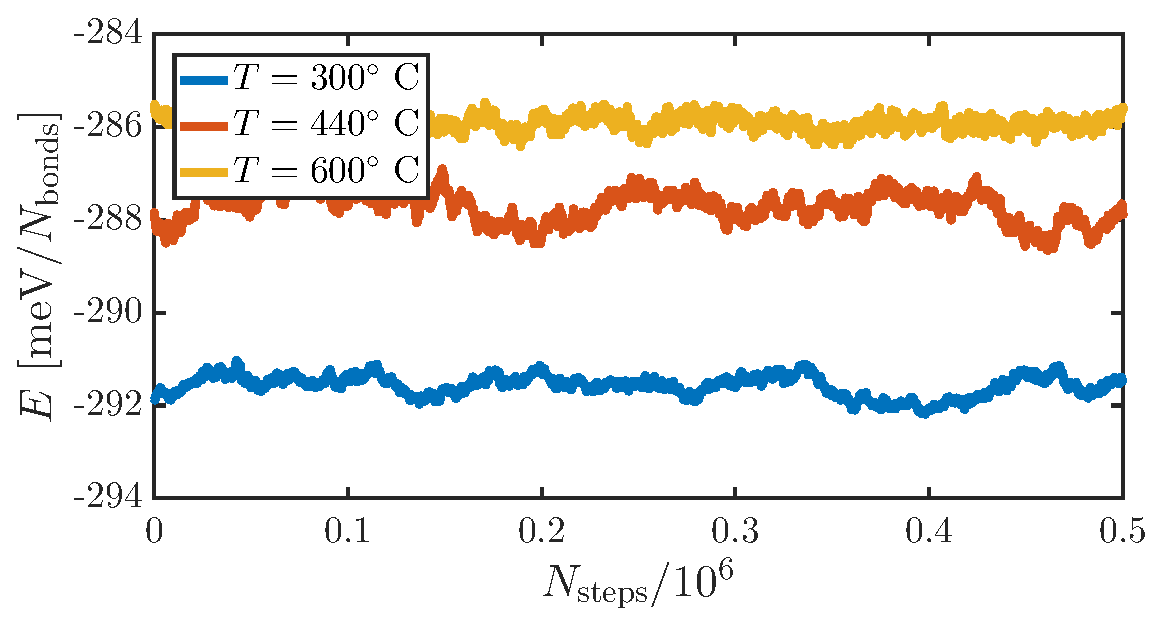
\includegraphics[width=0.7\textwidth]{../figures/equilibration} 
  \caption{The energy normalized to the number of bonds in the system during the equilibration process.}
  \label{fig:T2:equil}
\end{center}
\end{figure}

\subsection*{Statistical properties}
Figure~\ref{fig:U} shows the equilibrium energy per cell as a function of temperature, and compared to the mean field theory. We also show the error bars of two standard deviations using the statistical inefficiency  as calculated from the correlation function in section~\ref{sec:ns}. 


The metropolis simulation differs significantly from the mean free theory prediction; the critical temperature is significantly higher in the simulation and the mean energy continues to increase with temperature beyond the transition. 

\begin{figure}[!ht]
\begin{center}
  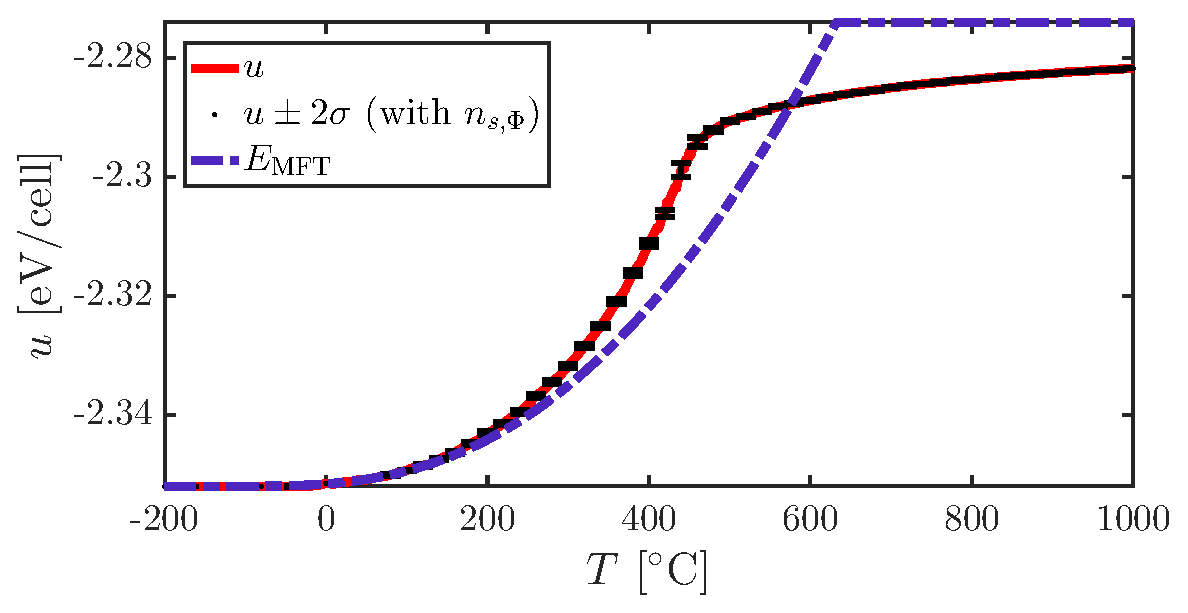
\includegraphics[width=0.7\textwidth]{../figures/U} 
  \caption{The average energy of the system normalized to the number of cells, as a function of temperature. Solid red: simulation, black: error bars at selected temperatures, dash-dotted blue: mean field theory prediction.}
  \label{fig:U}
\end{center}
\end{figure}

In mean field theory, the energy per cell never exceeds $8 E_0 = \unit[-2.31]{eV}$, but in the Monte Carlo simulation the system is allowed to develop clusters of Cu and Zn atoms, which gives a higher energy than the completely randomly ordered system. In the high temperature limit of an infinite system, the theoretical maximum energy is $ 8 E_{\rm max} \approx \unit[-2.276]{eV}$ (defined in equation~\eqref{eq:Emax}). With a limited system size with 10 cells in each direction, we estimate that the maximum energy should be approximately 
\begin{equation}
8 (0.9\cdot E_{\rm max} + 0.1 E_{\rm CuZn}) \approx \unit[2.284]{eV}
\end{equation}
Here we obtain $E \approx \unit[-2.287]{eV}$ at $\unit[600]{^\circ C}$, which is slightly below this limit. 

The heat capacity can be determined either by 
\begin{equation}
C = \frac{d U}{d T},
\label{eq:C1}
\end{equation}
or as the variance in the energy:
\begin{equation}
C = \frac{1}{k_{\rm B} T^2}\left(\langle E^2 \rangle  - \langle E \rangle^2 \right)
\label{eq:C2}.
\end{equation}
Since the latter method does not depend on the derivatives, it gives less noisy data. This is can be seen from figure~\ref{fig:C} by comparing the gray and the black lines. Again, we note that the mean field theory gives a lower critical temperature than the simulation. 

\begin{figure}[!ht]
\begin{center}
  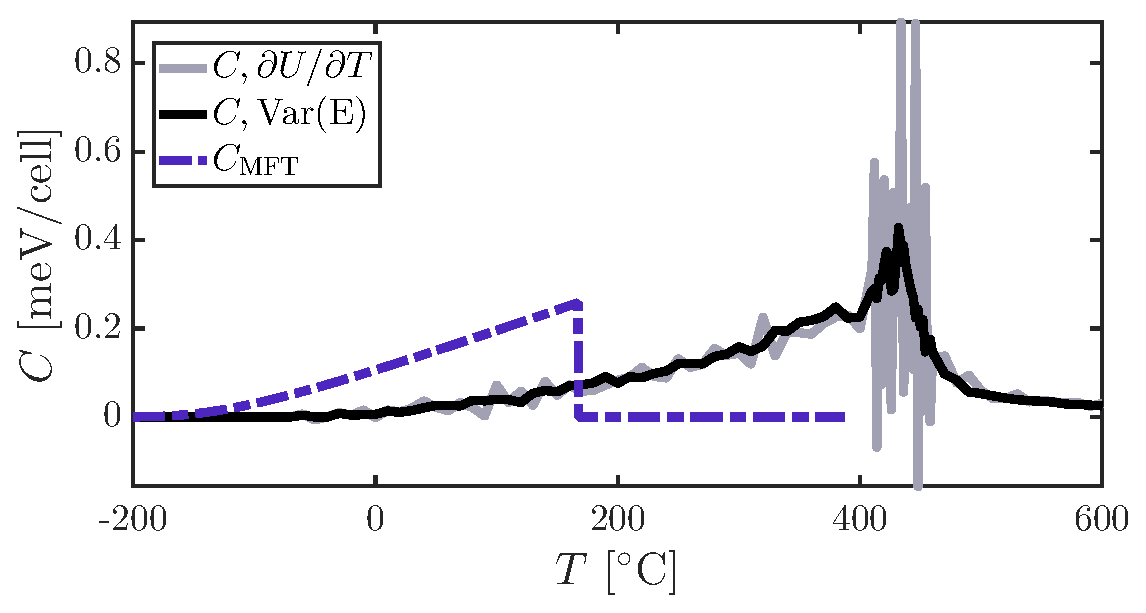
\includegraphics[width=0.7\textwidth]{../figures/C} 
  \caption{The specific heat of the system normalized to the number of cells, as a function of temperature. Solid gray: simulation using the derivative of $U$ directly, black: simulation using the variance of $E$, dash-dotted blue: mean field theory prediction.}
  \label{fig:C}
\end{center}
\end{figure}

\begin{figure}[!ht]
\begin{center}
  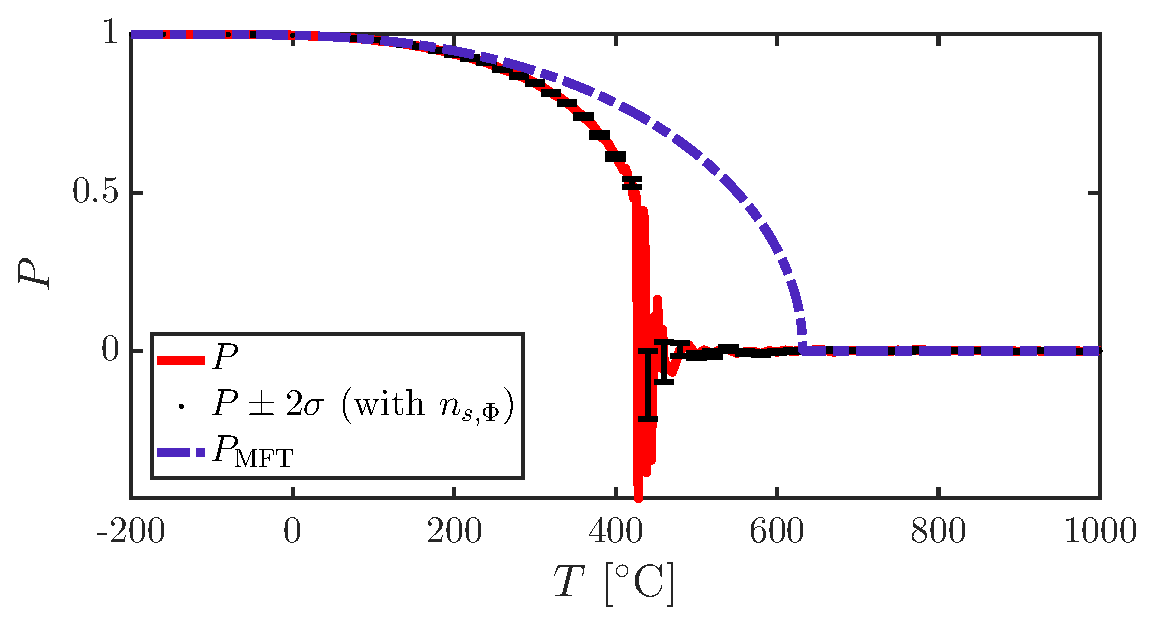
\includegraphics[width=0.7\textwidth]{../figures/P} 
  \caption{The order parameter $P$ as a function of temperature. Solid red: simulation, black: error bars at selected temperatures, dash-dotted blue: mean field theory prediction.}
  \label{fig:P}
\end{center}
\end{figure}

The order parameter $P$ is shown in figure~\ref{fig:P}. Close to the phase transition, the data has high uncertainty, which is also reflected in the large error bars. Note that $P <0$ at some temperature above the critical temperature -- the system oscillates between a majority of the Cu atoms in the Cu sublattice, and a majority in the Zn sublattice.  

Finally, the short range order parameter $r$ is determined by the number of nearest-neighbor Cu-Zn bonds $q$ as follows
\begin{equation}
r = \frac{1}{4 N}(q-4N) \rightarrow \begin{cases}
1, \quad {\rm perfect \, order} \\
0, \quad  {\rm no \, order, \, homogeneous \, system}\\
-1, \qquad {\rm fully \, separated \, system}
\end{cases}
\end{equation}
In the mean field theory, $r = P^2$. Figure~\ref{fig:r} therefore shows not only the simulation and the MFT prediction, but also the curve $P^2$. Until the transition, $r \approx P^2$ is a good estimation, but at higher temperatures $r$ remains non-zero despite $P \approx 0$. We speculate that this is a sign that there are still more Cu-Zn bonds than the homogeneous system without order. Just like there are clusters of Cu atoms and Zn atoms, there could be clusters of order, which could possibly explain this behavior. 

\begin{figure}[!ht]
\begin{center}
  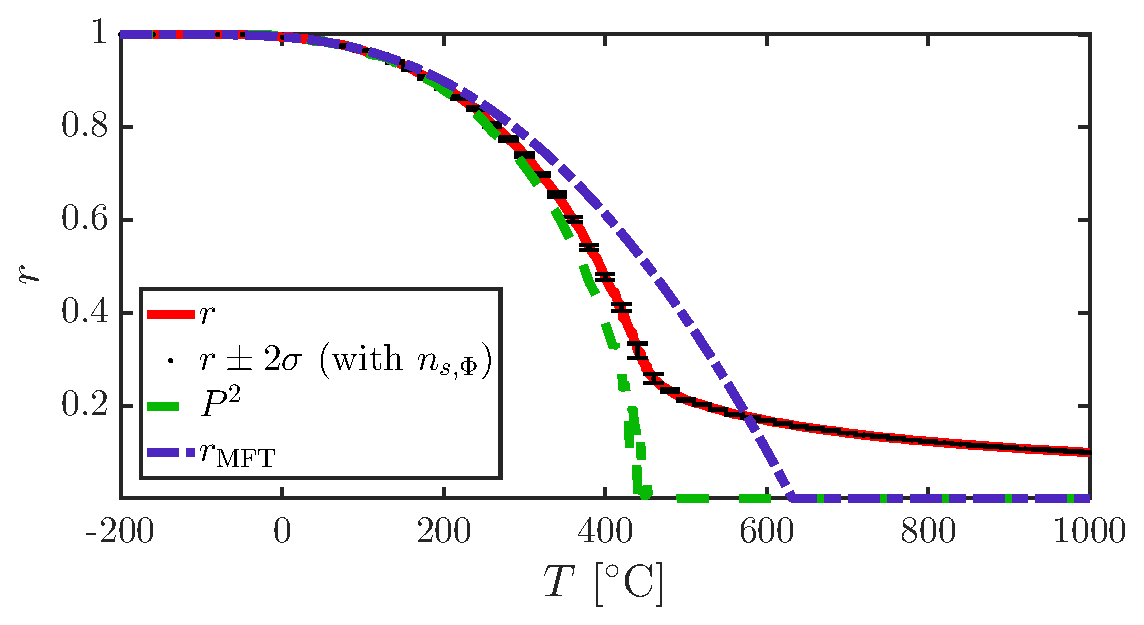
\includegraphics[width=0.7\textwidth]{../figures/r} 
  \caption{The short range order parameter as a function of temperature. Solid red: simulation, black: error bars at selected temperatures, dashed green: estimate $r \approx P^2$, dash-dotted blue: mean field theory prediction. }
  \label{fig:r}
\end{center}
\end{figure}




\subsection*{Statistical inefficiency}
\label{sec:ns}
As described in the Lecture notes, the statistical inefficiency can be used to obtain error estimates of correlated data. 

Suppose we want to measure a quantity $I$, as an average of $N\gg1$ measurements: 
\begin{equation}
I = \langle f \rangle \equiv \frac{1}{N}\sum_{i = 1}^N f_i.
\end{equation}

The variance is then given by 
\begin{equation}
{\rm Var}[I] = \frac{n_s}{N}{\rm Var}[f], \quad {\rm Var}[f] = \langle f^2 \rangle - \langle f \rangle^2,
\end{equation}
where $n_s$ is the statistical inefficiency. 
The statistical inefficiency can be determined either from the decay of the correlation function, 
\begin{equation}
\Phi_{k = n_s} = e^{-2} \approx 0.1, \quad \frac{\langle f_i f_{i+k}\rangle - \langle f \rangle^2}{\langle f^2\rangle - \langle f \rangle^2},
\label{eq:ns_Phi}
\end{equation}
or from block averaging
\begin{equation}
n_s = \lim_{B \rightarrow \infty} \frac{B {\rm Var}[F]}{{\rm Var}[f]}\,, \quad F_j = \frac{1}{B}\sum_{i = 1}^B f_{i + (j-1)B}\,, \quad j \in [1, N_{\rm blocks} ].
\label{eq:ns_block}
\end{equation}

The two methods in equations~\eqref{eq:ns_Phi} and~\eqref{eq:ns_block} should give similar estimates of $n_s$, which they do in the simulations here. The obtained statistical inefficiency is shown in figures~\ref{fig:ns_phi} and~\ref{fig:ns_block}   at three different temperatures, calculated with the correlation function and block average respectively. 

In the case of block average, we used a moving average of 100 points, as the data become noisy when the block size become comparable to the total number of steps. Alternatively, we could have made more blocks of the largest sizes by also using shifted blocks of data, but the results obtained here were considered accurate enough. 

\begin{figure}[!ht]
\begin{center}
  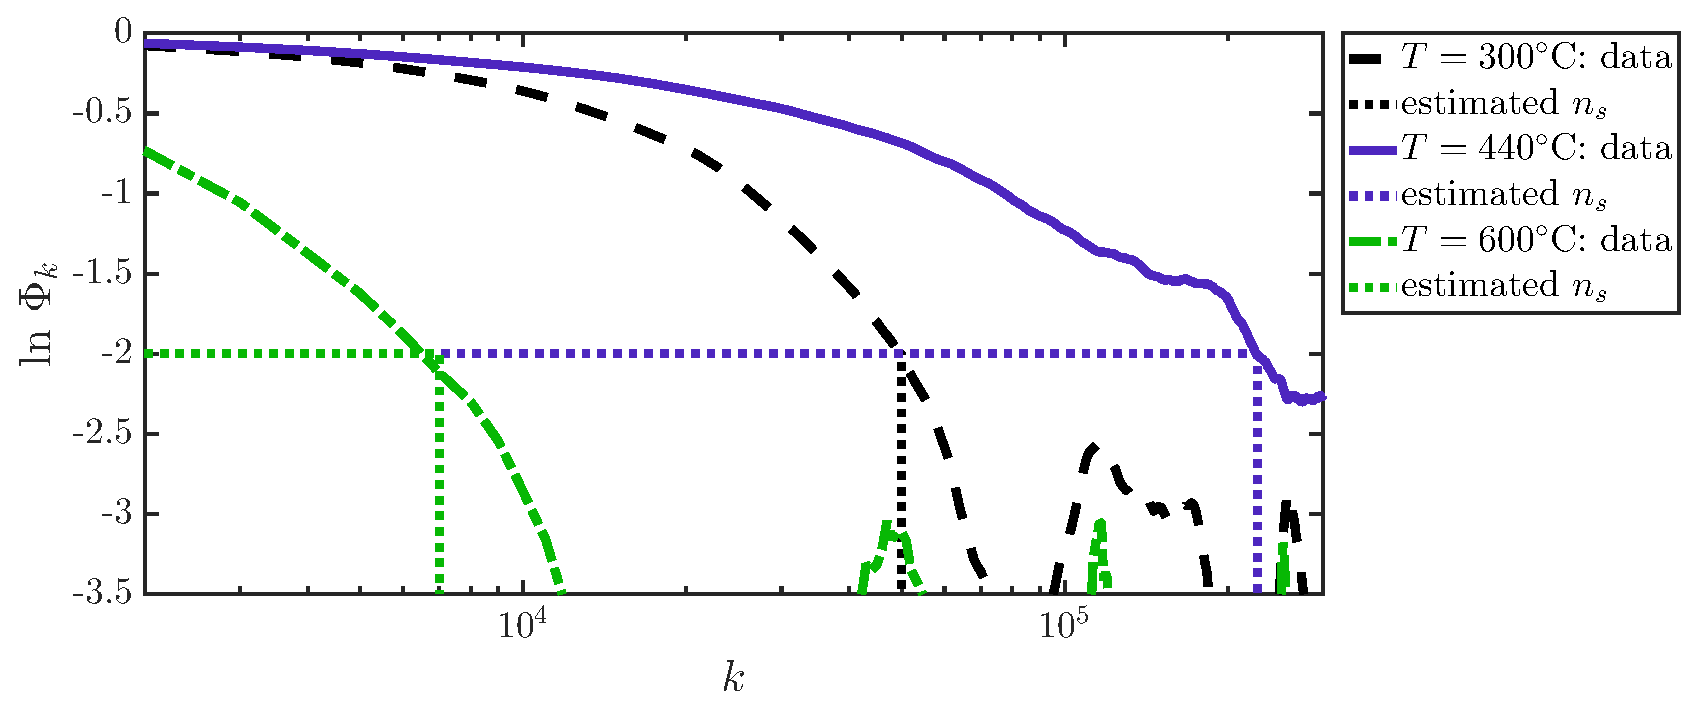
\includegraphics[width=\textwidth]{../figures/stat_inefficiency_Phi} 
  \caption{The logarirhm of the correlation function $\Phi_k(k)$ for three different temperatures. Dotted lines mark the estimated value of $n_s = k (\ln \Phi_k = -2)$.}
  \label{fig:ns_phi}
\end{center}
\end{figure}

\begin{figure}[!ht]
\begin{center}
  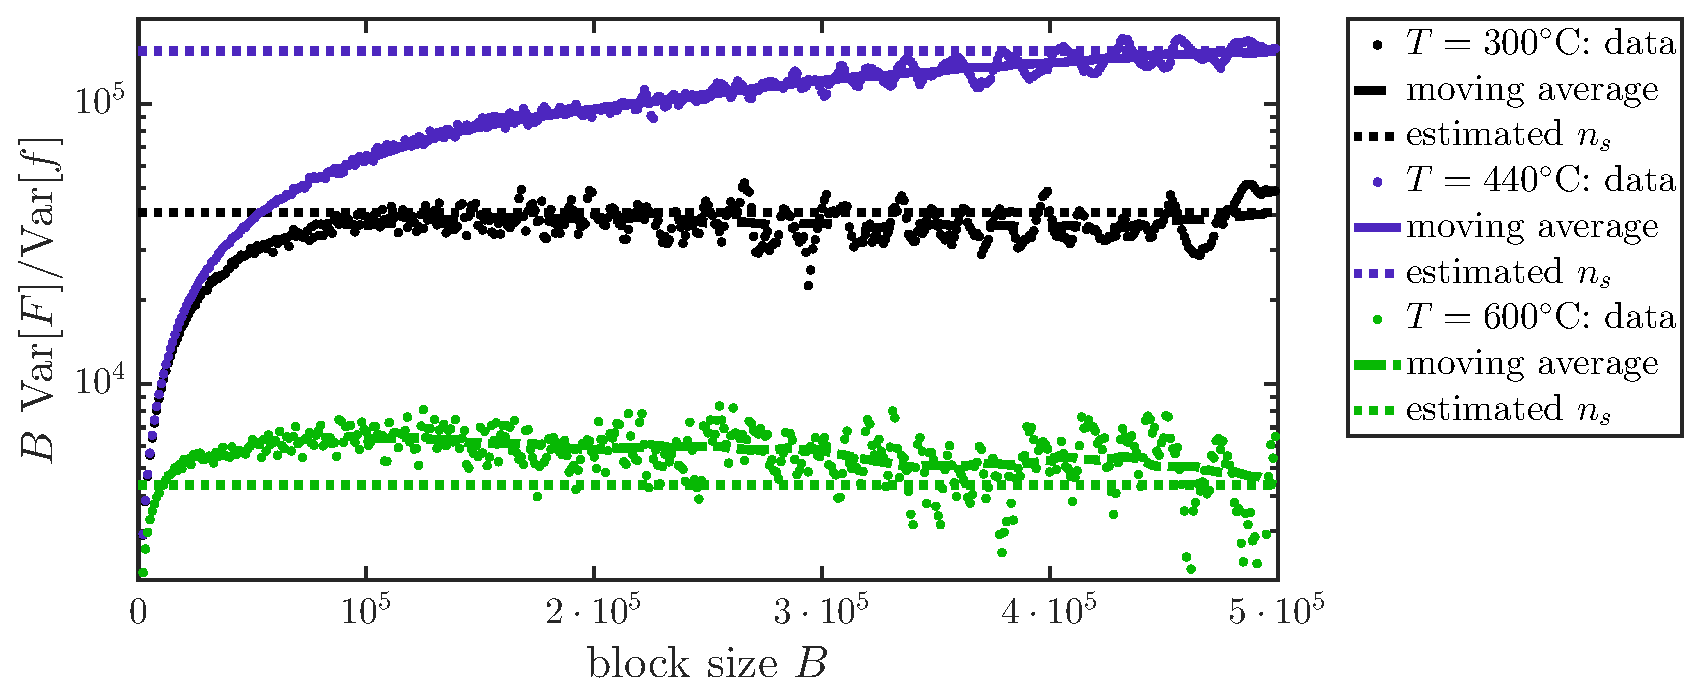
\includegraphics[width=\textwidth]{../figures/stat_inefficiency_block} 
  \caption{The statistical inefficiency determined with block averages for three different temperatures. Raw data is shown with dots, solid line show a moving average with 100 points, and the dotted lines show the estimated values of the statistical inefficiency.}
  \label{fig:ns_block}
\end{center}
\end{figure}

Note in figures~\ref{fig:ns_phi} and~\ref{fig:ns_block} that the statistical inefficiency is larger close to the phase transition at $T \approx \unit[440]{^\circ C}$ than at the lower and higher temperatures  $T = \unit[300]{^\circ C}$ and $T = \unit[600]{^\circ C}$. We speculate that this is related to the diverging property of the correlation length close to the phase transition. 

This peak in the statistical inefficiency close to the phase transition can be clearly identified also in figure~\ref{fig:ns_both}, where $n_s$ is plotted as a function of temperature using the two methods described above. We note that both methods give similar estimates of $n_s$, but the correlation function give larger fluctuations than the block average method. Moreover, we note that the statistical inefficiency diverges as $T \rightarrow \unit[0]{K}$. This is because very few changes in the lattice will be accepted at low temperatures, which give highly correlated data. At low temperatures, the equilibrium system is almost completely ordered, and we note that the uncertainty of the quantities $U, P$ and $r$ is still small at low temperatures as their variance decrease rapidly with decreasing temperature. 

\begin{figure}[!ht]
\begin{center}
  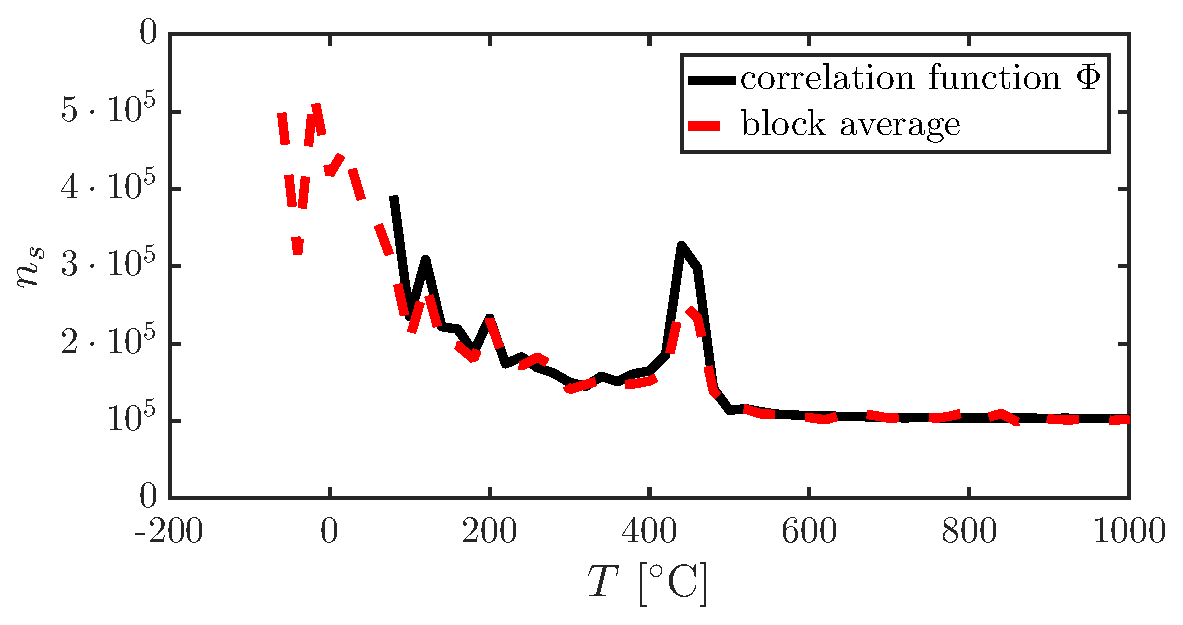
\includegraphics[width=0.7\textwidth]{../figures/stat_inefficiency_both} 
  \caption{The statistical inefficiency $n_s$ as a function of temperature using both the correlation function and block averages to determine $n_s$.}
  \label{fig:ns_both}
\end{center}
\end{figure}
\section*{Concluding discussion}
We study a binary alloy of brass. We compare semi-analytical results from mean-field theory with a Monte Carlo simulation using the Metropolis algorithm, and determine the energy, heat capacity, the order parameter as well as the short range order parameter. 
We find that the mean field theory underestimates the critical temperature and also fails to explain the behavior of the system above this phase transition. 
\newpage

\appendix

\section{Source Code}

%\subsection{Calculating pi using matlab: \texttt{pi.m}}
%\lstinputlisting[language=matlab,numbers=left]{template_files/pi.m}

%\subsection{Calculating pi using python: \texttt{pi.py}}
%\lstinputlisting[language=python,numbers=left]{template_files/pi.py}

\subsection{Main program task 2: \texttt{main\_T2.c}}
\lstinputlisting[language=c,numbers=left]{../code/main_T2.c}


\subsection{Misc functions : \texttt{funcs.c}}
\lstinputlisting[language=c,numbers=left]{../code/funcs.c}

\section{Auxiliary }
\subsection{Makefile}
\lstinputlisting[language=bash,numbers=left]{../code/Makefile}

\section{MATLAB scripts}
\subsection{Task 1 and analysis scripts for Task 2}
\lstinputlisting[language=matlab,numbers=left]{../m_scripts/H2_analysis.m}

\subsection{Improve figure appearance: \texttt{ImproveFigureCompPhys.m}}
\lstinputlisting[language=matlab,numbers=left]{../m_scripts/ImproveFigureCompPhys.m}

\subsection{Change size of figures: \texttt{setFigureSize.m}}
\lstinputlisting[language=matlab,numbers=left]{../m_scripts/setFigureSize.m}
\end{document}

%%% Local Variables:
%%% mode: latex
%%% TeX-master: t
%%% End:
